\section{Polynomial Multiplication II}
\begin{itemize}
	\item As a recap, we have two polynomials \( p \) and \( q \), both of degree \(  n -1 \), and we want to multiply 
		them. 
	\item We saw the \textit{coefficient representation}, where we specify its coefficients. So for \( p \), we have \( (p_0, p_1, 
		\dots, p_{n-1})\). Last lecture, we saw \( O(n^2) \) algorithm to multiply the polynomials using the 
		coefficient representation.
	\item We also saw the \textit{value representation}, where instead of giving the polynomial itself we give a set of 
		\( m \) points that the polynomial passes through. As long as \( m \ge  n \), then this set of points 
		fully specifies the polynomial. With this representation, we saw that polynomials can be multiplied in \( O(n) \) time. 
	\item So our main question was: is there a way for us to use the value representation to speed up the coefficient 
		representation multiplication?
	\item Roots of unity: the set of points we will evaluate our polynomials on. 
\end{itemize}
\subsection{Fast Fourier Transform}
\begin{itemize}
	\item Input: \( m \), a power of 2, a \( p(x) = p_0 + p_1x + \cdots + p_{m-1}x^{m-1} \). Our goal is to evaluate 
		 \( p( \omega_0), p(\omega_1), \dots, p(\omega_{m - 1}) \). 
	 \item We will use a divide and conquer approach:
		 \begin{center}
		 	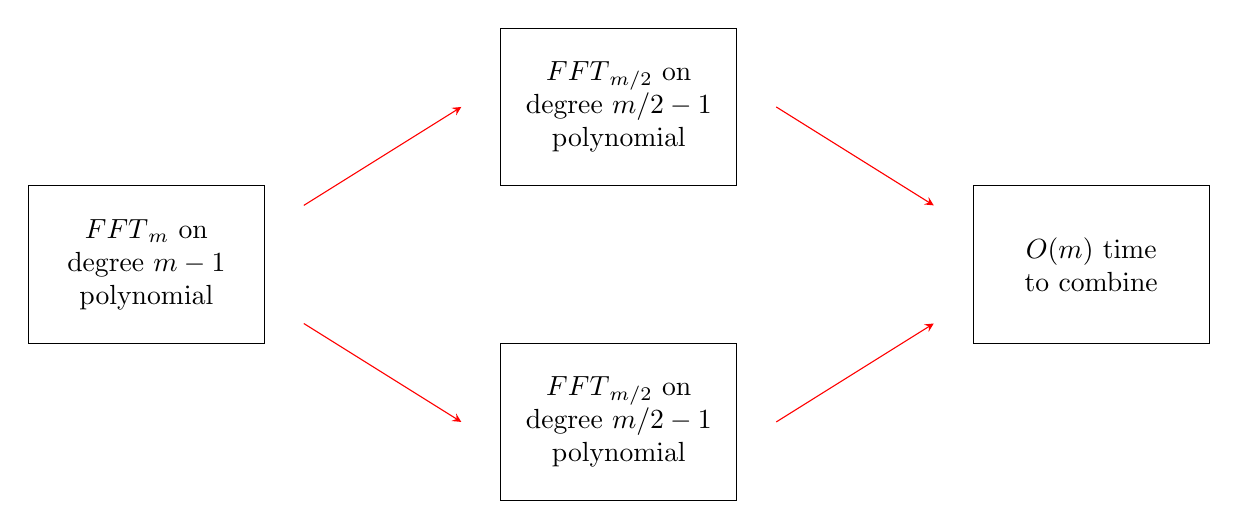
\begin{tikzpicture}[every text node part/.style={align=center}]
		 		\draw(0, -1) -- (3, -1) -- (3, 1) -- (0, 1) -- cycle;
				\draw(6, 1) -- (9, 1) -- (9, 3) -- (6, 3) -- cycle;
				\draw(6, -1) -- (9, -1) -- (9, -3) -- (6, -3) -- cycle;
				\draw(12, -1) -- (15, -1) -- (15, 1) -- (12, 1) -- cycle;
				\draw node at (1.5, 0) {\( \text{FFT}_m \) on \\degree \( m - 1 \) \\ polynomial}; 
				\draw node at (7.5, 2) { \( \text{FFT}_{m / 2} \) on \\ degree \( m / 2 - 1 \) \\ polynomial};
				\draw node at (7.5, -2) { \( \text{FFT}_{m / 2} \) on \\ degree \( m / 2 - 1 \) \\ polynomial};
				\draw node at (13.5, 0) {\( O(m) \) time \\ to combine};
				\draw[-stealth, red] (3.5, 0.75) -- (5.5, 2);
				\draw[-stealth, red] (3.5, -0.75) -- (5.5, -2);
				\draw[-stealth, red] (9.5, 2) -- (11.5, 0.75);
				\draw[-stealth, red] (9.5, -2) -- (11.5, -0.75); 
		 	\end{tikzpicture}
		 \end{center}
		 This will give us a recurrence relation \( T(m) \le  2 \cdot T(m / 2) + O(m) \), and from the master theorem this 
		 gives an \( O(m \log m) \) runtime.
\end{itemize}
\subsection{Divide and Conquer}
\begin{itemize}
	\item To figure out how to divide, let's first write out \( p(x) \) :
		\[
		p(x) = p_0 + p_1x + p_2x^2 + p_3x^3 + \cdots
		\] 
		Let's split \( p \) into two parts, based on the parity of the exponent. We'll call these the even and odd 
		halves:
		\begin{align*}
			p_E(x) &= p_0 + p_2x^2 + p_4x^{4} + \cdots + p_{m - 2}x^{m - 2}\\
			p_O(x) &= p_1x + p_3x^3 + \cdots + p_{m - 1} x^{m - 1} 
		\end{align*}
		But notice that we can rewrite the even part a little bit:
		\[
		p_E(x) = p_0 + p_2(x^2) + p_4(x^2)^2 + p_6(x^2)^3 + \cdots = \text{Even}(x^2)
		\] 
		But this looks like a polynomial with coefficietns \( p_0, p_2, p_4, \dots \) evaluated on \( x^2 \)! We will call 
		this polynomial \( \text{Even}(z) \). For the odd part, we factor out an \( x \) :
		\[
		p_1x + p_3x^3 + \cdots = x(p_1 + p_3x^2 + p_5x^{4} + \cdots) = x \cdot \text{Odd}(x^2)
		\] 
		The key to note here is that we have a recursion in the fact that we can express the evaluation of the polynomials 
		at the \( n \)-th step as a computation involving another polynomial but evaluated on \( x^2 \). So, we have 
		\[
		p(x) = \text{Even}(x^2) + x \cdot \text{Odd}(x^2)
		\] 
		The degree of the even part is \( (m - 2) / 2 = m / 2 - 1 \), and the same goes for odd part.   
	\item Now if we want to compute \( p \) on \( \omega_i \), then we have \( p(\omega_i) = \text{Even}(\omega_i^2) + 
		\omega_i \cdot \text{Odd}(\omega_i^2)\). 
	\item Because we are squaring the arguments, then this means that we are evaluating the Even and Odd parts on the 
		\( m / 2 \)-th roots of unity, because of our magical fact!
	\item So to compute \( p(\omega_i) \), we recursively evaluate the even and odd parts at the  \( m / 2 \)-th roots of unity:
		\( \alpha_0, \alpha_1, \dots, \alpha_{m / 2 - 1} \). 
	\item To combine, all we need to do is multiply the odd part by  \( \omega_i \), then add the two parts together. So, the 
		combination step only takes \( O(m) \) work. So this fully gives our recursion \( T(m) \le  2 \cdot T(m / 2) + O(m) \), 
		hence the \( O(m \log m) \) runtime. 
\end{itemize}
\subsection{Fast Interpolation}
\begin{itemize}
	\item An update on our algorithm scheme:
		\begin{center}
			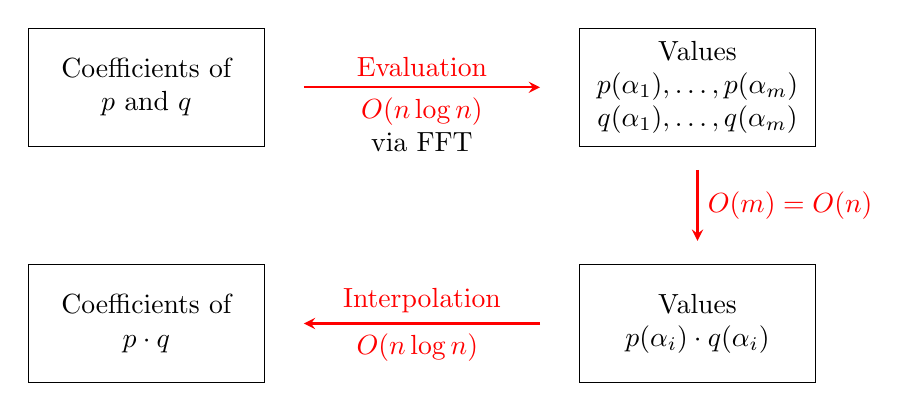
\begin{tikzpicture}[every text node part/.style={align=center}]
				\foreach \x in {0, 7}
				\foreach \y in {0, 3}
				{
					\draw (\x, \y) -- (\x+3, \y) -- (\x+3, \y+1.5) -- (\x, \y+1.5) -- cycle;
				}
				\draw node at (1.5, 0.75) {Coefficients of \\ \( p \cdot q \)};
				\draw node at (1.5, 3.75) {Coefficients of \\ \( p \) and \( q \) };
				\draw node at (8.5, 0.75) {Values \\ \( p(\alpha_i) \cdot q(\alpha_i) \) };
				\draw node at (8.5, 3.75) {Values \\ \( p(\alpha_1), \dots, p(\alpha_m) \) \\ \( q(\alpha_1), \dots, q(\alpha_m) \) };
				\draw[-stealth, red, thick] (3.5, 3.75) --node[midway, above] {Evaluation} node[midway, below] 
					{\( O(n \log n) \) \\ \textcolor{black}{via FFT}} (6.5, 3.75); 
				\draw[-stealth, red, thick] (8.5, 2.7) -- node[midway, right] {\( O(m) = O(n) \) } (8.5, 1.8);
				\draw[-stealth, red, thick] (6.5, 0.75) -- node[midway, above] {Interpolation} node[midway, below] 
					{\( O(n \log n) \) } (3.5, 0.75);
			\end{tikzpicture}
		\end{center}
	\item Now we want to figure out the interpolation step: given \( r(\omega_0), r(\omega_1), \dots, r(\omega_{m - 1}) \), we want 
		to get back the coefficient representation of \( r(x) \). This is called the inverse FFT. 
	\item It turns out that when we do the Fourier transform, we basically get the inverse Fourier transform for free. Recall 
		the Fourier transform:
		\[
			p(\omega_\ell) = \sum_{j = 0}^{m - 1}p_j (\omega_\ell)^{j}
		\]
		This equation comes from replacing all \( x \) 's with \( \omega_\ell \). Then, the inverse Fourier transform is written 
		as follows:
		\[
			p_{\ell} = \frac{1}{m} \cdot \sum_{j = 0}^{m - 1}p(\omega_j) \cdot (\omega_{m - \ell})^{j} = \frac{1}{m} \cdot 
			q(\omega_{m - \ell})
		\] 
		Here, \( q(x) = p(\omega_0) + p(\omega_1)x + \cdots p(\omega_{m - 1})x^{m - 1} \). So in essence, this is basically another 
		polynomial evaluation, which we already know happens in \( O(m \log m) = O(n \log n) \) time!
	\item So, now let's look at the completed diagram:
		\begin{center}
			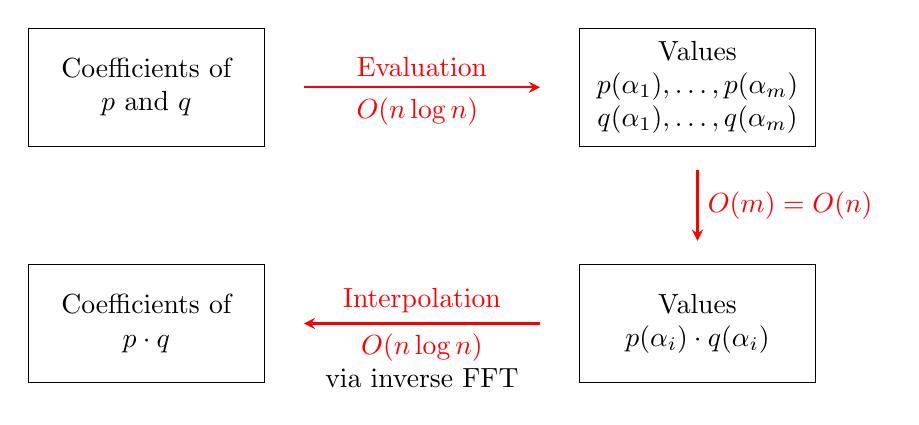
\begin{tikzpicture}[every text node part/.style={align=center}]
				\foreach \x in {0, 7}
				\foreach \y in {0, 3}
				{
					\draw (\x, \y) -- (\x+3, \y) -- (\x+3, \y+1.5) -- (\x, \y+1.5) -- cycle;
				}
				\draw node at (1.5, 0.75) {Coefficients of \\ \( p \cdot q \)};
				\draw node at (1.5, 3.75) {Coefficients of \\ \( p \) and \( q \) };
				\draw node at (8.5, 0.75) {Values \\ \( p(\alpha_i) \cdot q(\alpha_i) \) };
				\draw node at (8.5, 3.75) {Values \\ \( p(\alpha_1), \dots, p(\alpha_m) \) \\ \( q(\alpha_1), \dots, q(\alpha_m) \) };
				\draw[-stealth, red, thick] (3.5, 3.75) --node[midway, above] {Evaluation} node[midway, below] 
					{\( O(n \log n) \) } (6.5, 3.75); 
				\draw[-stealth, red, thick] (8.5, 2.7) -- node[midway, right] {\( O(m) = O(n) \) } (8.5, 1.8);
				\draw[-stealth, red, thick] (6.5, 0.75) -- node[midway, above] {Interpolation} node[midway, below] 
					{\( O(n \log n) \) \\ \textcolor{black}{via inverse FFT}} (3.5, 0.75);
			\end{tikzpicture}
		\end{center}
		So this shows that polynomial multiplication can be done in \( O(n \log n) \) time!  
\end{itemize}
\subsection{The Matrix Viewpoint}
\begin{itemize}
	\item There's another way to represent \( p(x) \), as a column vector:
		\[
		\begin{bmatrix} p(\omega_0)\\p(\omega_1)\\p(\omega_2)\\ \vdots \\ p(\omega_{m - 1}) \end{bmatrix} = 
		\begin{bmatrix} p_0 + p_1\omega_0 + p_2 \omega_0^2 + \cdots + p_{m-1}\omega_0^{m- 1}\\
		p_0 + p_1 \omega_1 + p_2\omega_1^2 + \cdots + p_{m-1}\omega_1^{m-1}\\
	\vdots \\
p_0 + p_1\omega_{m-1} + p_2\omega_{m-1}^2 + \cdots+ p_{m-1}\omega_{m-1}^{m-1}\end{bmatrix} 
= \underbrace{\begin{bmatrix} 1 & \omega_0 & \omega_0^2 & \dots & \omega_0^{m-1}\\
1 & \omega_1 & \omega_1^2 & \dots & \omega_1^{m-1}\\
1 & \omega_2 & \omega_2^2 & \dots & \omega_2^{m-1}\\
\vdots & \vdots & \vdots & \ddots & \vdots\\
1 & \omega_{m-1} & \omega_{m-1}^2 & \dots & \omega_{m-1}^{m-1}\end{bmatrix}}_{M} \cdot \underbrace{\begin{bmatrix} p_0\\p_1\\p_2\\ \vdots \\p_{m-1} \end{bmatrix}}_{[p]} 
		\] 
	\item If we didn't know FFT, then this computation is just a matrix multiplied by a vector, whihc would take \( O(m^2) \)  
		time. However, FFT basically gives us a way to compute this matrix in \( O(m \log m) \) time!

		Note also that this also solves this \textbf{without ever writing down \( M \) !} 
	\item The Inverse FFT looks much cleaner in this representation:
		\[
		M^{-1} \cdot \begin{bmatrix} p(\omega_0)\\p(\omega_1)\\p(\omega_2)\\ \vdots \\ p(\omega_{m-1}) \end{bmatrix} = 
		\begin{bmatrix} p_0\\p_1\\p_2\\ \vdots \\ p_{m-1} \end{bmatrix} 
		\] 
	\item For \( M \) specifically, we have \( M_{ij} = \omega_i^{j} = (\omega_1^{i})^{j} = \omega_1^{ij} \). Then, the inverse 
		is defined as: \( (M^{-1})_{ij} = \frac{1}{n} \cdot \omega_{m-i}^{j} \). 
\end{itemize}
\subsection{Applications}
\begin{itemize}
	\item \textbf{Cross Correlation:}
		Given the product of \( p(x) = p_0 + p_1x + p_2x^2 + p_3x^3 \) and \( q(x) = q_0 + q_1x + q_2x^2 + q_3x^3 \), the 
		coefficient on \( x^{i} \) in \( p(x) \cdot q(x) \) is
		\[
		p_0q_{i} + p_1q_{i-1} + \cdots + p_{i-1}q_{1} + p_{i}q_0
		\] 
		Now consider two arrays \( [p_0, p_1, p_2, p_3] \) and \( [q_3, q_2, q_1, q_0] \). Now let's stack them on top of each 
		other and take the dot product of the overlap. Depending on where they overlap, it actually corresponds to the coefficient 
		on some \( x^{i} \) in \( p(x) \cdot q(x) \).  
		\begin{center}
			\includegraphics[scale=0.5]{cross-correlation.png}
		\end{center}
		This is called \textbf{cross-correlation}, and due to FFT, we can compute these in \( O(n \log n) \) time.   
	\item  \textbf{Integer Multiplication:} Say we wanted to multiply \( a = a_{n-1} \cdots a_2a_1a_0 \) and 
		\( b = b_{n-1}\cdots b_2b_1b_0 \). We can write down these two polynomials:
		\begin{align*}
			A &= a_0 + a_1x + a_2x^2 + \cdots + a_{n-1}x^{n-1}\\
			B&= b_0 + b_1x + b_2x^2 + \cdots + b_{n-1}x^{n-1} 
		\end{align*}
		and to compute the product, we can write \( A(x) \cdot B(x) \) and plug in \( x = 10 \). Naively we would think that 
		this takes \( O(n \log n) \) time, but this is not exactly true. This is because here, our additions and multiplications 
		don't exactly happen in \( O(1) \) time anymore, so we have to be careful! In fact, the multiplication can be as 
		large as \( \Theta(n) \). 

		After keeping track of all this, we get an \( O(n \log n \log \log n) \) algorithm. 
	\item \textbf{Fourier Transform:} FFT allows us to compute the Fourier transform of \( p(x) \) quickly -- we can decompose 
		 \( p(x) \) into its consistuent sines and cosines. There are too many applications of the Fourier transform to 
		 even list: 
		 \begin{enumerate}[label=\arabic*.]
		 	\item Music software
			\item Heart rate monitor
			\item Signal processing (e.g. cell phones)
			\item Many more!
		 \end{enumerate}
		 The fact that quantum computers can compute Fourier transforms exceedingly quickly is actually one of the main reasons 
		 that makes them so powerful.
\end{itemize}
